

\documentclass[10pt]{article}

%\usepackage[cp1251]{inputenc}

\usepackage[english,russian]{babel}

\usepackage{amsmath}

\usepackage{amssymb}

\usepackage{amsfonts}

\usepackage{chngcntr,color}

%\usepackage[hyper]{amsbib}

\usepackage{ulem}

\usepackage[hidelinks]{hyperref}

\usepackage[mathscr]{euscript}

\usepackage{enumitem}

\usepackage{cite}

\usepackage{bbm} % We need this for pretty Indicator \mathbbm{1}.

\usepackage[left=25mm, top=20mm, right=10mm, bottom=10mm, nohead]{geometry}

    \usepackage{graphicx} % для картинок





\renewcommand\theequation{\arabic{section}.\arabic{equation}}

\newcommand{\ra}{\rightarrow}

\newcommand{\p}[1]{{\mathbf{P}} \left( \, #1 \, \right) }

\newcommand{\px}[1]{{\mathbf{P}_x}\!\left( \, #1 \, \right) }

\newcommand{\e}{{\mathbf{E}} }

\newcommand{\lk}{«}

\newcommand{\pk}{»}

\newcommand{\lm}{(\lambda,\mu)}

\newcommand{\sk}[1]{\left[ #1 \right]}

\newcommand{\skk}[1]{\left\{ #1 \right\}}

\newcommand{\lef}{\left(}

\newcommand{\rig}{\right)}

\newcommand{\skl}[1]{\left\langle #1 \right\rangle}



\renewcommand{\le}{\leqslant}

\renewcommand{\ge}{\geqslant}



 \def\lms{\mathop{\overline{\lim}}\limits}



\def\lmi{\mathop{\underline{\lim}}\limits}



\def\v{\varepsilon}



\def\d{\delta}

\def\a{\alpha}

\def\b{\beta}

\def\g{\gamma}

\def\l{\lambda}

\def\m{\mu}

\def\({\left(}

\def\){\right)}



\def\({\left(}

\def\){\right)}



\def\[{\left[}

\def\]{\right]}





\def\|{\left|}

\def\|{\right|}







\def\SL{\left\{}

\def\SP{\right\}}



\def\dd{{\boldsymbol{\delta}}}

\def\aa{{\boldsymbol{\alpha}}}

\def\bb{{\boldsymbol{\beta}}}

\def\gg{{\boldsymbol{\gamma}}}

\def\ll{{\boldsymbol{lambda}}}

\def\mm{{\boldsymbol{\mu}}}

\def\0{{\boldsymbol{0}}}





\def\n{\nu}

\def\t{\tau}

\def\x{\xi}

\def\z{\zeta}

\def\zz{{\boldsymbol{\zeta}}}

\def\e{\eta}

\def\h{\theta}

\def\ll{{\boldsymbol{\lambda}}}

\def\mm{{\boldsymbol{\mu}}}

\def\xx{{\boldsymbol{\xi}}}

\def\ppsi{{\boldsymbol{\psi}}}

\def\LL{{\boldsymbol{\Lambda}}}







\def\DD{Д\ о\ к\ а\ з\ а\ т\ е\ л\ ь\ с\ т\ в\ о}

\def\D{\mathbb D}

\def\C{\mathbb C}

\def\R{\mathbb R}

\def\Z{\mathbb Z}

\def\V{\mathbb V}





\def\r{\rho}

\def\x{\xi}



\pagestyle{empty} 



%    \raisebox{-1pt}[0pt][0pt]{
\includegraphics[width=0.02\linewidth]{3.png}}

\begin{document} 
\begin{center} {\Large Билет №1} \end{center} 

\raisebox{-1pt}[0pt][0pt]{
\includegraphics[width=0.02\linewidth]{3.png}} Опр.( сигма – алгебры). Примеры сигма-алгебр. \\

\raisebox{-1pt}[0pt][0pt]{
\includegraphics[width=0.02\linewidth]{3.png}} Опр (носителя случайной величины). \\

\raisebox{-1pt}[0pt][0pt]{
\includegraphics[width=0.02\linewidth]{3.png}} Лемма (вычисление УМО для а.н.р.)  (без док-ва). \\

\raisebox{-1pt}[0pt][0pt]{
\includegraphics[width=0.02\linewidth]{3.png}} Опр. (простой случайной величины). \\

\raisebox{-1pt}[0pt][0pt]{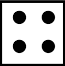
\includegraphics[width=0.02\linewidth]{4.png}} Теорема (формула Бернулли). Доказательство. \\

\raisebox{-1pt}[0pt][0pt]{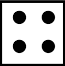
\includegraphics[width=0.02\linewidth]{4.png}} Контрпример не нормального вектора с нормальными одномерными компонентами. Доказательство. \\ 

\raisebox{-1pt}[0pt][0pt]{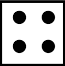
\includegraphics[width=0.02\linewidth]{4.png}} Следствие (о независимости и корреляции для нормального вектора). Доказательство. \\

\raisebox{-1pt}[0pt][0pt]{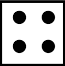
\includegraphics[width=0.02\linewidth]{4.png}}   Пример сингулярного распределения (лестница Кантора). \\

\raisebox{-1pt}[0pt][0pt]{
\includegraphics[width=0.02\linewidth]{5.png}} Теорема Слуцкого. Доказательство. \\

\raisebox{-1pt}[0pt][0pt]{
\includegraphics[width=0.02\linewidth]{5.png}}  Теорема (о квантильном преобразование). Доказательство. \\

\raisebox{-1pt}[0pt][0pt]{
\includegraphics[width=0.02\linewidth]{5.png}} Теорема (об эквивалентных определениях независимости). Доказательство. \\

\raisebox{-1pt}[0pt][0pt]{
\includegraphics[width=0.02\linewidth]{5.png}} Теорема (по вероятности vs слабая). Доказательство. \\  

\begin{center} {\Large Билет №2} \end{center} 

\raisebox{-1pt}[0pt][0pt]{
\includegraphics[width=0.02\linewidth]{3.png}} Аксиомы дискретной вероятности. Примеры. \\

\raisebox{-1pt}[0pt][0pt]{
\includegraphics[width=0.02\linewidth]{3.png}} Опр. (коэффициента корреляции Кендалла). \\

\raisebox{-1pt}[0pt][0pt]{
\includegraphics[width=0.02\linewidth]{3.png}} Опр. (многомерного нормального распределения). Вид плотности для многомерного стандартного нормального вектора. \\ 

\raisebox{-1pt}[0pt][0pt]{
\includegraphics[width=0.02\linewidth]{3.png}} Теорема (неравенство Маркова). (без док-ва) \\

\raisebox{-1pt}[0pt][0pt]{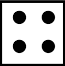
\includegraphics[width=0.02\linewidth]{4.png}} Следствие (о независимости и корреляции для нормального вектора). Доказательство. \\ 

\raisebox{-1pt}[0pt][0pt]{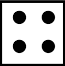
\includegraphics[width=0.02\linewidth]{4.png}} Основные свойства математического ожидания с доказательством (Однородность, монотонность, нер-во треугольника, аддитивность). \\

\raisebox{-1pt}[0pt][0pt]{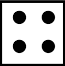
\includegraphics[width=0.02\linewidth]{4.png}} Теорема (о плотности). Доказательство. \\

\raisebox{-1pt}[0pt][0pt]{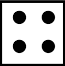
\includegraphics[width=0.02\linewidth]{4.png}} Теорема (формула полной вероятности). Доказательство. \\

\raisebox{-1pt}[0pt][0pt]{
\includegraphics[width=0.02\linewidth]{5.png}} Вычисление интеграла от плотности нормального распределения.  Свойства нормального распределения с доказательством (лин. преобр., равенства для $\Phi_{0,1},$ правило трех сигм). \\

\raisebox{-1pt}[0pt][0pt]{
\includegraphics[width=0.02\linewidth]{5.png}}   Теорема (о квантилях и линейном преобазование случайных величин, обобщенная обратная функция). Доказательство. \\

\raisebox{-1pt}[0pt][0pt]{
\includegraphics[width=0.02\linewidth]{5.png}} Теорема (о линейном преобразование для нормального вектора). Доказательство. \\

\raisebox{-1pt}[0pt][0pt]{
\includegraphics[width=0.02\linewidth]{5.png}} Теорема (УМО для гауссовских векторов). Доказательство. \\

\begin{center} {\Large Билет №3} \end{center} 

\raisebox{-1pt}[0pt][0pt]{
\includegraphics[width=0.02\linewidth]{3.png}}   Опр. (квантили в общей случае). \\

\raisebox{-1pt}[0pt][0pt]{
\includegraphics[width=0.02\linewidth]{3.png}} Опр. (смешанного распределения). Примеры. \\

\raisebox{-1pt}[0pt][0pt]{
\includegraphics[width=0.02\linewidth]{3.png}} Опр. (пространства элементарных исходов), примеры пространств элементарных исходов и событий. \\

\raisebox{-1pt}[0pt][0pt]{
\includegraphics[width=0.02\linewidth]{3.png}} Опр. (абсолютно непрерывного распределения). Примеры. \\

\raisebox{-1pt}[0pt][0pt]{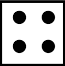
\includegraphics[width=0.02\linewidth]{4.png}} Лемма (вычисление УМО для а.н.р.). Доказательство. \\

\raisebox{-1pt}[0pt][0pt]{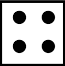
\includegraphics[width=0.02\linewidth]{4.png}} Свойства ковариации с доказательством. \\

\raisebox{-1pt}[0pt][0pt]{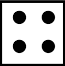
\includegraphics[width=0.02\linewidth]{4.png}} Теорема (Шкляра). Доказательство в непрерывном случае. \\

\raisebox{-1pt}[0pt][0pt]{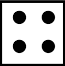
\includegraphics[width=0.02\linewidth]{4.png}} Пример (парадокс Бертрана). \\ 

\raisebox{-1pt}[0pt][0pt]{
\includegraphics[width=0.02\linewidth]{5.png}} Свойства коэффициента корреляции с доказательством. \\

\raisebox{-1pt}[0pt][0pt]{
\includegraphics[width=0.02\linewidth]{5.png}} Теорема об ортогональной проекции. Доказательство. \\

\raisebox{-1pt}[0pt][0pt]{
\includegraphics[width=0.02\linewidth]{5.png}} Теорема (Бореля-Кантелли). Доказательство. \\

\raisebox{-1pt}[0pt][0pt]{
\includegraphics[width=0.02\linewidth]{5.png}}  Теорема (о квантильном преобразование). Доказательство. \\

\begin{center} {\Large Билет №4} \end{center} 

\raisebox{-1pt}[0pt][0pt]{
\includegraphics[width=0.02\linewidth]{3.png}} Опр. (сингулярного распределения). Примеры. \\

\raisebox{-1pt}[0pt][0pt]{
\includegraphics[width=0.02\linewidth]{3.png}} Замечание (о вычисление  математического ожидания для преобразований случайных величин (одномерных и многомерных преобразований)). \\

\raisebox{-1pt}[0pt][0pt]{
\includegraphics[width=0.02\linewidth]{3.png}} Опр. (логнормального распределения). Вычисление плотности. \\

\raisebox{-1pt}[0pt][0pt]{
\includegraphics[width=0.02\linewidth]{3.png}} Опр. (многомерного нормального распределения). Вид плотности для многомерного стандартного нормального вектора. \\ 

\raisebox{-1pt}[0pt][0pt]{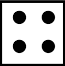
\includegraphics[width=0.02\linewidth]{4.png}}  Пример (Бернштейна). \\

\raisebox{-1pt}[0pt][0pt]{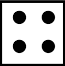
\includegraphics[width=0.02\linewidth]{4.png}} Классическое неравенство Чебышёва. Доказательство. \\

\raisebox{-1pt}[0pt][0pt]{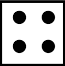
\includegraphics[width=0.02\linewidth]{4.png}} Свойства матрицы ковариации (при линейном преобразование, для суммы независимых случайных векторов). Доказательство. \\

\raisebox{-1pt}[0pt][0pt]{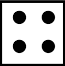
\includegraphics[width=0.02\linewidth]{4.png}} Теорема (Шкляра). Доказательство в непрерывном случае. \\

\raisebox{-1pt}[0pt][0pt]{
\includegraphics[width=0.02\linewidth]{5.png}} Свойства УМО с доказательством (УМО по более бедной сигма алгебре, вынос измеримой с.в. ). \\

\raisebox{-1pt}[0pt][0pt]{
\includegraphics[width=0.02\linewidth]{5.png}} Теорема (полиномиальная схема). Доказательство. \\

\raisebox{-1pt}[0pt][0pt]{
\includegraphics[width=0.02\linewidth]{5.png}} Теорема об ортогональной проекции. Доказательство. \\

\raisebox{-1pt}[0pt][0pt]{
\includegraphics[width=0.02\linewidth]{5.png}} Свойства коэффициентов корреляции Спирмена и Кендалла. Доказательство. \\ 

\begin{center} {\Large Билет №5} \end{center} 

\raisebox{-1pt}[0pt][0pt]{
\includegraphics[width=0.02\linewidth]{3.png}} Опр. (смешанного распределения). Примеры. \\

\raisebox{-1pt}[0pt][0pt]{\includegraphics[width=0.02\linewidth]{3.png}} Опр. (сингулярного распределения). Примеры. \\

\raisebox{-1pt}[0pt][0pt]{\includegraphics[width=0.02\linewidth]{3.png}} Опр. (сходимости по вероятности). \\

\raisebox{-1pt}[0pt][0pt]{\includegraphics[width=0.02\linewidth]{3.png}} Опр. (абсолютно непрерывного распределения). Примеры. \\

\raisebox{-1pt}[0pt][0pt]{\includegraphics[width=0.02\linewidth]{4.png}} Свойства многомерного математического ожидания (линейность, произведение независимых матриц). Доказательство. \\ 

\raisebox{-1pt}[0pt][0pt]{\includegraphics[width=0.02\linewidth]{4.png}} Теорема (центральная предельная теорема). Доказательство. \\        

\raisebox{-1pt}[0pt][0pt]{\includegraphics[width=0.02\linewidth]{4.png}} Лемма (вычисление УМО для дискретных). Доказательство. \\

\raisebox{-1pt}[0pt][0pt]{\includegraphics[width=0.02\linewidth]{4.png}} Свойства функций распределения с доказательствами. \\

\raisebox{-1pt}[0pt][0pt]{\includegraphics[width=0.02\linewidth]{5.png}} Теорема (п.н. vs по вероятности). Доказательство. \\

\raisebox{-1pt}[0pt][0pt]{\includegraphics[width=0.02\linewidth]{5.png}}  Свойство счетной аддитивности математического ожидания. Доказательство. \\

\raisebox{-1pt}[0pt][0pt]{\includegraphics[width=0.02\linewidth]{5.png}} Теорема (об инвариантности копулы при строго возрастающем преобразовании). Доказательство. \\

\raisebox{-1pt}[0pt][0pt]{\includegraphics[width=0.02\linewidth]{5.png}} Свойства коэффициента корреляции с доказательством. \\

\begin{center} {\Large Билет №6} \end{center} 

\raisebox{-1pt}[0pt][0pt]{\includegraphics[width=0.02\linewidth]{3.png}} Теорема (с.к.с. vs p vs п.н.) (без док-ва). \\ 

\raisebox{-1pt}[0pt][0pt]{\includegraphics[width=0.02\linewidth]{3.png}} Опр. (дискретного распределения). Примеры. \\

\raisebox{-1pt}[0pt][0pt]{\includegraphics[width=0.02\linewidth]{3.png}} Замечание (о вычисление  математического ожидания для дискретных, для а.н.р). \\

\raisebox{-1pt}[0pt][0pt]{\includegraphics[width=0.02\linewidth]{3.png}} Опр. (борелевской сигма-алгебра). \\

\raisebox{-1pt}[0pt][0pt]{\includegraphics[width=0.02\linewidth]{4.png}} Теорема (свертка для дискретных). Доказательство. \\

\raisebox{-1pt}[0pt][0pt]{\includegraphics[width=0.02\linewidth]{4.png}} Замечание (о неулучшаемости неравенства Берри-Эссеена). \\

\raisebox{-1pt}[0pt][0pt]{\includegraphics[width=0.02\linewidth]{4.png}} Свойства матрицы ковариации (при линейном преобразование, для суммы независимых случайных векторов). Доказательство. \\

\raisebox{-1pt}[0pt][0pt]{\includegraphics[width=0.02\linewidth]{4.png}} Следствие (о независимости и корреляции для нормального вектора). Доказательство. \\

\raisebox{-1pt}[0pt][0pt]{\includegraphics[width=0.02\linewidth]{5.png}} Теорема (оценка точности в теореме Пуассона). Доказательство. \\

\raisebox{-1pt}[0pt][0pt]{\includegraphics[width=0.02\linewidth]{5.png}} Свойства характеристических функций с доказательством (значение в нуле, линейное преобразование, сумма независимых, гладкость в нуле). \\

\raisebox{-1pt}[0pt][0pt]{\includegraphics[width=0.02\linewidth]{5.png}} Теорема (об эквивалентных определениях независимости). Доказательство. \\

\raisebox{-1pt}[0pt][0pt]{\includegraphics[width=0.02\linewidth]{5.png}} Теорема (УМО для гауссовских векторов). Доказательство. \\

\begin{center} {\Large Билет №7} \end{center} 

\raisebox{-1pt}[0pt][0pt]{\includegraphics[width=0.02\linewidth]{3.png}} Лемма (вычисление УМО для а.н.р.)  (без док-ва). \\

\raisebox{-1pt}[0pt][0pt]{\includegraphics[width=0.02\linewidth]{3.png}} Опр. (независимых случайных величин). \\

\raisebox{-1pt}[0pt][0pt]{\includegraphics[width=0.02\linewidth]{3.png}} Опр. (гауссовской копулы). \\

\raisebox{-1pt}[0pt][0pt]{\includegraphics[width=0.02\linewidth]{3.png}} Теорема (неравенство Маркова). (без док-ва) \\

\raisebox{-1pt}[0pt][0pt]{\includegraphics[width=0.02\linewidth]{4.png}} Свойства ковариации с доказательством. \\

\raisebox{-1pt}[0pt][0pt]{\includegraphics[width=0.02\linewidth]{4.png}} Лемма (вычисление УМО для дискретных). Доказательство. \\

\raisebox{-1pt}[0pt][0pt]{\includegraphics[width=0.02\linewidth]{4.png}} Свойства совместной функции распределения. Доказательство. \\

\raisebox{-1pt}[0pt][0pt]{\includegraphics[width=0.02\linewidth]{4.png}} Теорема (о сохранение независимости при преобразованиях). Доказательство. \\ 

\raisebox{-1pt}[0pt][0pt]{\includegraphics[width=0.02\linewidth]{5.png}} Теорема (полиномиальная схема). Доказательство. \\

\raisebox{-1pt}[0pt][0pt]{\includegraphics[width=0.02\linewidth]{5.png}} Теорема Слуцкого. Доказательство. \\

\raisebox{-1pt}[0pt][0pt]{\includegraphics[width=0.02\linewidth]{5.png}} Теорема (п.н. vs по вероятности). Доказательство. \\

\raisebox{-1pt}[0pt][0pt]{\includegraphics[width=0.02\linewidth]{5.png}} Свойства характеристических функций с доказательством (значение в нуле, линейное преобразование, сумма независимых, гладкость в нуле). \\

\begin{center} {\Large Билет №8} \end{center} 

\raisebox{-1pt}[0pt][0pt]{\includegraphics[width=0.02\linewidth]{3.png}} Опр. (пространства элементарных исходов), примеры пространств элементарных исходов и событий. \\

\raisebox{-1pt}[0pt][0pt]{\includegraphics[width=0.02\linewidth]{3.png}} Следствие об устойчивости по суммированию (без док-ва). \\

\raisebox{-1pt}[0pt][0pt]{\includegraphics[width=0.02\linewidth]{3.png}}   Опр. (квантили для непрерывной функции распределения). \\

\raisebox{-1pt}[0pt][0pt]{\includegraphics[width=0.02\linewidth]{3.png}} Опр. (коэффициента корреляции Спирмена). \\

\raisebox{-1pt}[0pt][0pt]{\includegraphics[width=0.02\linewidth]{4.png}} Свойства вероятностной меры с доказательствами (вероятность пустого мн-ва, дизъюнктного объединения, дополнения, объединения двух мн-в, монотонность). \\

\raisebox{-1pt}[0pt][0pt]{\includegraphics[width=0.02\linewidth]{4.png}} Теорема (Шкляра). Доказательство в непрерывном случае. \\

\raisebox{-1pt}[0pt][0pt]{\includegraphics[width=0.02\linewidth]{4.png}} Свойства совместной функции распределения. Доказательство. \\

\raisebox{-1pt}[0pt][0pt]{\includegraphics[width=0.02\linewidth]{4.png}} Теорема (формула Байеса). Доказательство. \\

\raisebox{-1pt}[0pt][0pt]{\includegraphics[width=0.02\linewidth]{5.png}} Теорема (о свертке для произвольных распределений). Доказательство. Следствие об а.н.р. суммы. \\ 

\raisebox{-1pt}[0pt][0pt]{\includegraphics[width=0.02\linewidth]{5.png}} Вычисление интеграла от плотности нормального распределения.  Свойства нормального распределения с доказательством (лин. преобр., равенства для $\Phi_{0,1},$ правило трех сигм). \\

\raisebox{-1pt}[0pt][0pt]{\includegraphics[width=0.02\linewidth]{5.png}} Свойства  вероятностной меры с доказательством (вероятность объединения счетного набора, непрерывность вер. меры, формула включения/исключения). \\

\raisebox{-1pt}[0pt][0pt]{\includegraphics[width=0.02\linewidth]{5.png}} Свойства коэффициентов корреляции Спирмена и Кендалла. Доказательство. \\ 

\begin{center} {\Large Билет №9} \end{center} 

\raisebox{-1pt}[0pt][0pt]{\includegraphics[width=0.02\linewidth]{3.png}} Опр.( сигма – алгебры). Примеры сигма-алгебр. \\

\raisebox{-1pt}[0pt][0pt]{\includegraphics[width=0.02\linewidth]{3.png}} Опр. (сходимости почти наверное). \\

\raisebox{-1pt}[0pt][0pt]{\includegraphics[width=0.02\linewidth]{3.png}} Опр. (сингулярного распределения). Примеры. \\

\raisebox{-1pt}[0pt][0pt]{\includegraphics[width=0.02\linewidth]{3.png}}  Опр. (показательного распределения). Доказательство, что это действительно распределение. Свойство нестарения. Вычисление функции распределения.  \\  

\raisebox{-1pt}[0pt][0pt]{\includegraphics[width=0.02\linewidth]{4.png}} Следствие (из ЦПТ). \\

\raisebox{-1pt}[0pt][0pt]{\includegraphics[width=0.02\linewidth]{4.png}} Теорема (центральная предельная теорема). Доказательство. \\        

\raisebox{-1pt}[0pt][0pt]{\includegraphics[width=0.02\linewidth]{4.png}} Свойства УМО с доказательством (УМО константы, УМО от измеримой с.в., монотонность,  линейность, неравенство треугольника,  аналог формулы полной вероятности). \\

\raisebox{-1pt}[0pt][0pt]{\includegraphics[width=0.02\linewidth]{4.png}} Классическое неравенство Чебышёва. Доказательство. \\

\raisebox{-1pt}[0pt][0pt]{\includegraphics[width=0.02\linewidth]{5.png}} Теорема (по вероятности vs слабая). Доказательство. \\  

\raisebox{-1pt}[0pt][0pt]{\includegraphics[width=0.02\linewidth]{5.png}} Теорема (о правой границе неравенства Frechet-Hoeffding).  Доказательство. \\

\raisebox{-1pt}[0pt][0pt]{\includegraphics[width=0.02\linewidth]{5.png}} Теорема об ортогональной проекции. Доказательство. \\

\raisebox{-1pt}[0pt][0pt]{\includegraphics[width=0.02\linewidth]{5.png}} Теорема (оценка точности в теореме Пуассона). Доказательство. \\

\begin{center} {\Large Билет №10} \end{center} 

\raisebox{-1pt}[0pt][0pt]{\includegraphics[width=0.02\linewidth]{3.png}}  Опр. (распределения Пуассона). Доказательство, что это действительно распределение. \\

\raisebox{-1pt}[0pt][0pt]{\includegraphics[width=0.02\linewidth]{3.png}} Опр. (вырожденного распределения). Пример случайных экспериментов и случайной величины с этим распределением. \\

\raisebox{-1pt}[0pt][0pt]{\includegraphics[width=0.02\linewidth]{3.png}}  Опр. (биномиального распределения). Доказательство, что это действительно распределение. Пример случайных экспериментов и случайной величины с этим распределением. \\     

\raisebox{-1pt}[0pt][0pt]{\includegraphics[width=0.02\linewidth]{3.png}} Опр. (Схемы Бернулли). Примеры экспериментов со схемой Бернулли. \\

\raisebox{-1pt}[0pt][0pt]{\includegraphics[width=0.02\linewidth]{4.png}} Свойства совместной функции распределения. Доказательство. \\

\raisebox{-1pt}[0pt][0pt]{\includegraphics[width=0.02\linewidth]{4.png}} Следствие (о независимости и корреляции для нормального вектора). Доказательство. \\ 

\raisebox{-1pt}[0pt][0pt]{\includegraphics[width=0.02\linewidth]{4.png}} Теорема (обобщенное неравенство Чебышёва). Доказательство. \\

\raisebox{-1pt}[0pt][0pt]{\includegraphics[width=0.02\linewidth]{4.png}} Свойства УМО с доказательством (УМО константы, УМО от измеримой с.в., монотонность,  линейность, неравенство треугольника,  аналог формулы полной вероятности). \\

\raisebox{-1pt}[0pt][0pt]{\includegraphics[width=0.02\linewidth]{5.png}} Теорема (по вероятности vs слабая). Доказательство. \\  

\raisebox{-1pt}[0pt][0pt]{\includegraphics[width=0.02\linewidth]{5.png}} Теорема (об инвариантности копулы при строго возрастающем преобразовании). Доказательство. \\

\raisebox{-1pt}[0pt][0pt]{\includegraphics[width=0.02\linewidth]{5.png}} Теорема (Бореля-Кантелли). Доказательство. \\

\raisebox{-1pt}[0pt][0pt]{\includegraphics[width=0.02\linewidth]{5.png}} Вычисление интеграла от плотности нормального распределения.  Свойства нормального распределения с доказательством (лин. преобр., равенства для $\Phi_{0,1},$ правило трех сигм). \\

\end{document}